\documentclass{article}

% if you need to pass options to natbib, use, e.g.:
%     \PassOptionsToPackage{numbers, compress}{natbib}
% before loading neurips_2018

% ready for submission
% \usepackage{neurips_2018}

% to compile a preprint version, e.g., for submission to arXiv, add add the
% [preprint] option:
%     \usepackage[preprint]{neurips_2018}

% to compile a camera-ready version, add the [final] option, e.g.:
     \usepackage[final]{neurips_2018}

% to avoid loading the natbib package, add option nonatbib:
%     \usepackage[nonatbib]{neurips_2018}

\usepackage[utf8]{inputenc} % allow utf-8 input
\usepackage[T1]{fontenc}    % use 8-bit T1 fonts
\usepackage{hyperref}       % hyperlinks
\usepackage{url}            % simple URL typesetting
\usepackage{booktabs}       % professional-quality tables
\usepackage{amsfonts}       % blackboard math symbols
\usepackage{nicefrac}       % compact symbols for 1/2, etc.
\usepackage{microtype}      % microtypography
\setcounter{secnumdepth}{0}
\usepackage{graphicx}
\usepackage{float}
\usepackage{subfigure}
\usepackage{subfig}

    
\title{LAB 1 - EL2805}

% The \author macro works with any number of authors. There are two commands
% used to separate the names and addresses of multiple authors: \And and \AND.
%
% Using \And between authors leaves it to LaTeX to determine where to break the
% lines. Using \AND forces a line break at that point. So, if LaTeX puts 3 of 4
% authors names on the first line, and the last on the second line, try using
% \AND instead of \And before the third author name.

\author{%
  Mustafa Al-Janabi \\
  970101-5035 \\
  \texttt{musaj@kth.se} \\
  \And  
  Mikel Zhobro \\
  950216-T590 \\
  \texttt{zhobro@kth.se} \\
  }

\begin{document}
% \nipsfinalcopy is no longer used

\maketitle

\section{Problem 1: The Maze and the Random Minotaur}
\subsection{a) MDP formulation}
\subsubsection{State space}
We define a state as a tuple (i,j,k,l) where the two first parameters describe the position of the player in the grid and the last two that of the minotaur. While the position of the player is restricted only on free grid spaces, the position of the minotaur can be everywhere on the grid map. In addition to that we define two terminal states which 
correspond to the state where the player is eaten by the minotaur and the state where the player has exited the maze successfully. The formal definition of the state space is given below.

\begin{equation} 
\label{state_space_1}
\mathcal{S} = \Big\lbrace (i,j,k,l) ~:  (i,j) \textrm{ is neither obstacle nor goal and } (i,j)\neq (k,l) \Big\rbrace  \cup \Big\lbrace Eaten \Big\rbrace \cup \Big\lbrace Exit\Big\rbrace
\end{equation}

\subsubsection{Action space $\mathcal{A}$}
The action space is defined as 
\begin{equation}
    \mathcal{A} = \{stay, up, down, left, right \}
\end{equation}

\subsubsection{Transition probabilities $\mathcal{P}$}
Two different models have been studied with respect to the transition probabilities.
\par 
\textbf{Model 1}
\par
In the first model the following set up is used for the transition 
probabilities.

\begin{itemize}
  \item Terminal state $ s = Eaten: P(s|s,a) = 1, P(s'|s,a) = 0 \textrm{ if } s' \neq s,  \forall a$.
  
  \item Terminal state $s = Exit:  P(s|s,a) = 1, P(s'|s,a) = 0 \textrm{ if } s' \neq s,  \forall a$.
  \item Player moves to empty cell $P(s'|s,a) = 1$
  \item Player moves to impossible cell $P(s'|s,a) = 0$
\end{itemize}
\par 
\textbf{Model 2}
\par
Since we did consider the random movement of the monotaur in the transition probabilities for this model, there is no need to penalize the positions near the minotaur as before. 
\begin{itemize}
  \item Terminal state $s=Eaten: P(s|s,a) = 1, P(s'|s,a) = 0, \textrm{ if } s' \neq s, \forall a $
  \item Terminal state $s=Exit: P(s|s,a) = 1, P(s'|s,a) = 0, \textrm{ if } s' \neq s, \forall a $
  \item Player takes action a, where next state, $s'$ is not an obstacle: \\
  $P(s'|s,a) = \frac{1}{\textrm{\#actions by minotaur}}  \forall s'$
  \item Player cannot move to obstacle $P(s'|s,a) = 0$ and must stay in place  $P(s|s,a) = 1$
  \item If next state $s'$ is an obstacle then the player stays in the same cell, ie. $P(s'|s,a)=0$ and $P(s|s,a)=1$
\end{itemize}

This change takes into account the fact that the minotaur makes a uniformly random move for every action.

\subsubsection{Rewards $\mathcal{R}$}
\textbf{Model 1}
\par
Since we didn't consider the random movements of the minotaur in the translation probabilities, this model solved that by giving a negative reward to the states where the player is located at a state which is immediately reachable by the minotaur. That is summarized by the following:
\begin{itemize}
    \item If at state $s$, taking action $a$ leads to a wall or an obstacle then $r(s,a) = -\infty$
    \item If at state $s$, taking action $a$ leads to the minotaur then $ r(s,a) = -80 $
    \item If at state $s$, taking action $a$ leads to a state where the player is at a state that is immediately reachable by the minotaur  $ r(s,a) = \frac{-80}{\textrm{\#actions by minotaur}}$
    \item If at state $s$ and previous state was with the minotaur, $r(s,a)=-80$
    \item If at state $s$, taking action $a$ leads to the exit then $ r(s,a) = 0 $
    \item If at state $s$ and previous state was the minotaur, $r(s,a)=0$
    \item If at state $s$, taking action $a$ leads to neither of the aforementioned states $ r(s,a) = -1 $
\end{itemize}

\textbf{Model 2}
\par
For this model we don't assume any different any reward for being in the moving range of the minotaur since the random movement of the minotaur is considered in the transition probabilities.
\begin{itemize}
    \item If at state $s$, taking action $a$ leads to a wall or an obstacle then $r(s,a) = -\infty$
    \item If at state $s$, taking action $a$ leads to the minotaur then $ r(s,a) = -80 $
    \item If at state $s$ and previous state was with the minotaur, $r(s,a)=-80$
    \item If at state $s$, taking action $a$ leads to the exit then $ r(s,a) = 0 $
    \item If at state $s$, taking action $a$ leads to neither of the aforementioned states $ r(s,a) = -1 $
\end{itemize}

\subsection{b) Solving the problem with finite horizon}
Firstly, we present an illustration of an optimal policy with time horizon $T=20$ in Figure (\ref{fig:1b-optpol})

\begin{figure}[ht]
  \centering
  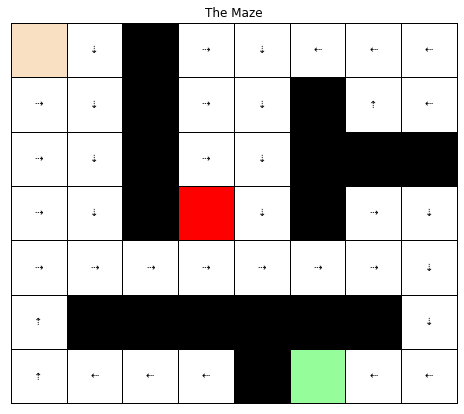
\includegraphics[width=0.9\linewidth]{img/optimalpolicyT20.png}
  \caption{The optimal policy shown as arrows given the player is in state $s=(i,j)=(0,0)$ and the minotaur at $s=(k,l)=(3,3)$  at time step t=0 with T=50.}
  \label{fig:1b-optpol}
\end{figure}

Secondly, we now study the probability of existing as a function of time, $T$. As discussed earlier, we denote the model where the minotaur is modeled in reward as \textbf{Model 1} and the model where the minotaur is described in the transition probabilities as \textbf{Model 2}. Furthermore we try two different scenarios, one where the minotaur only take the actions: $up, left, down, right$. And another scenario where the minotaur can also take the action $stay$ on top of $up, down, right, left$. The result is presented in Figure (\ref{fig:1b}).

\begin{figure}[ht]
  \centering

  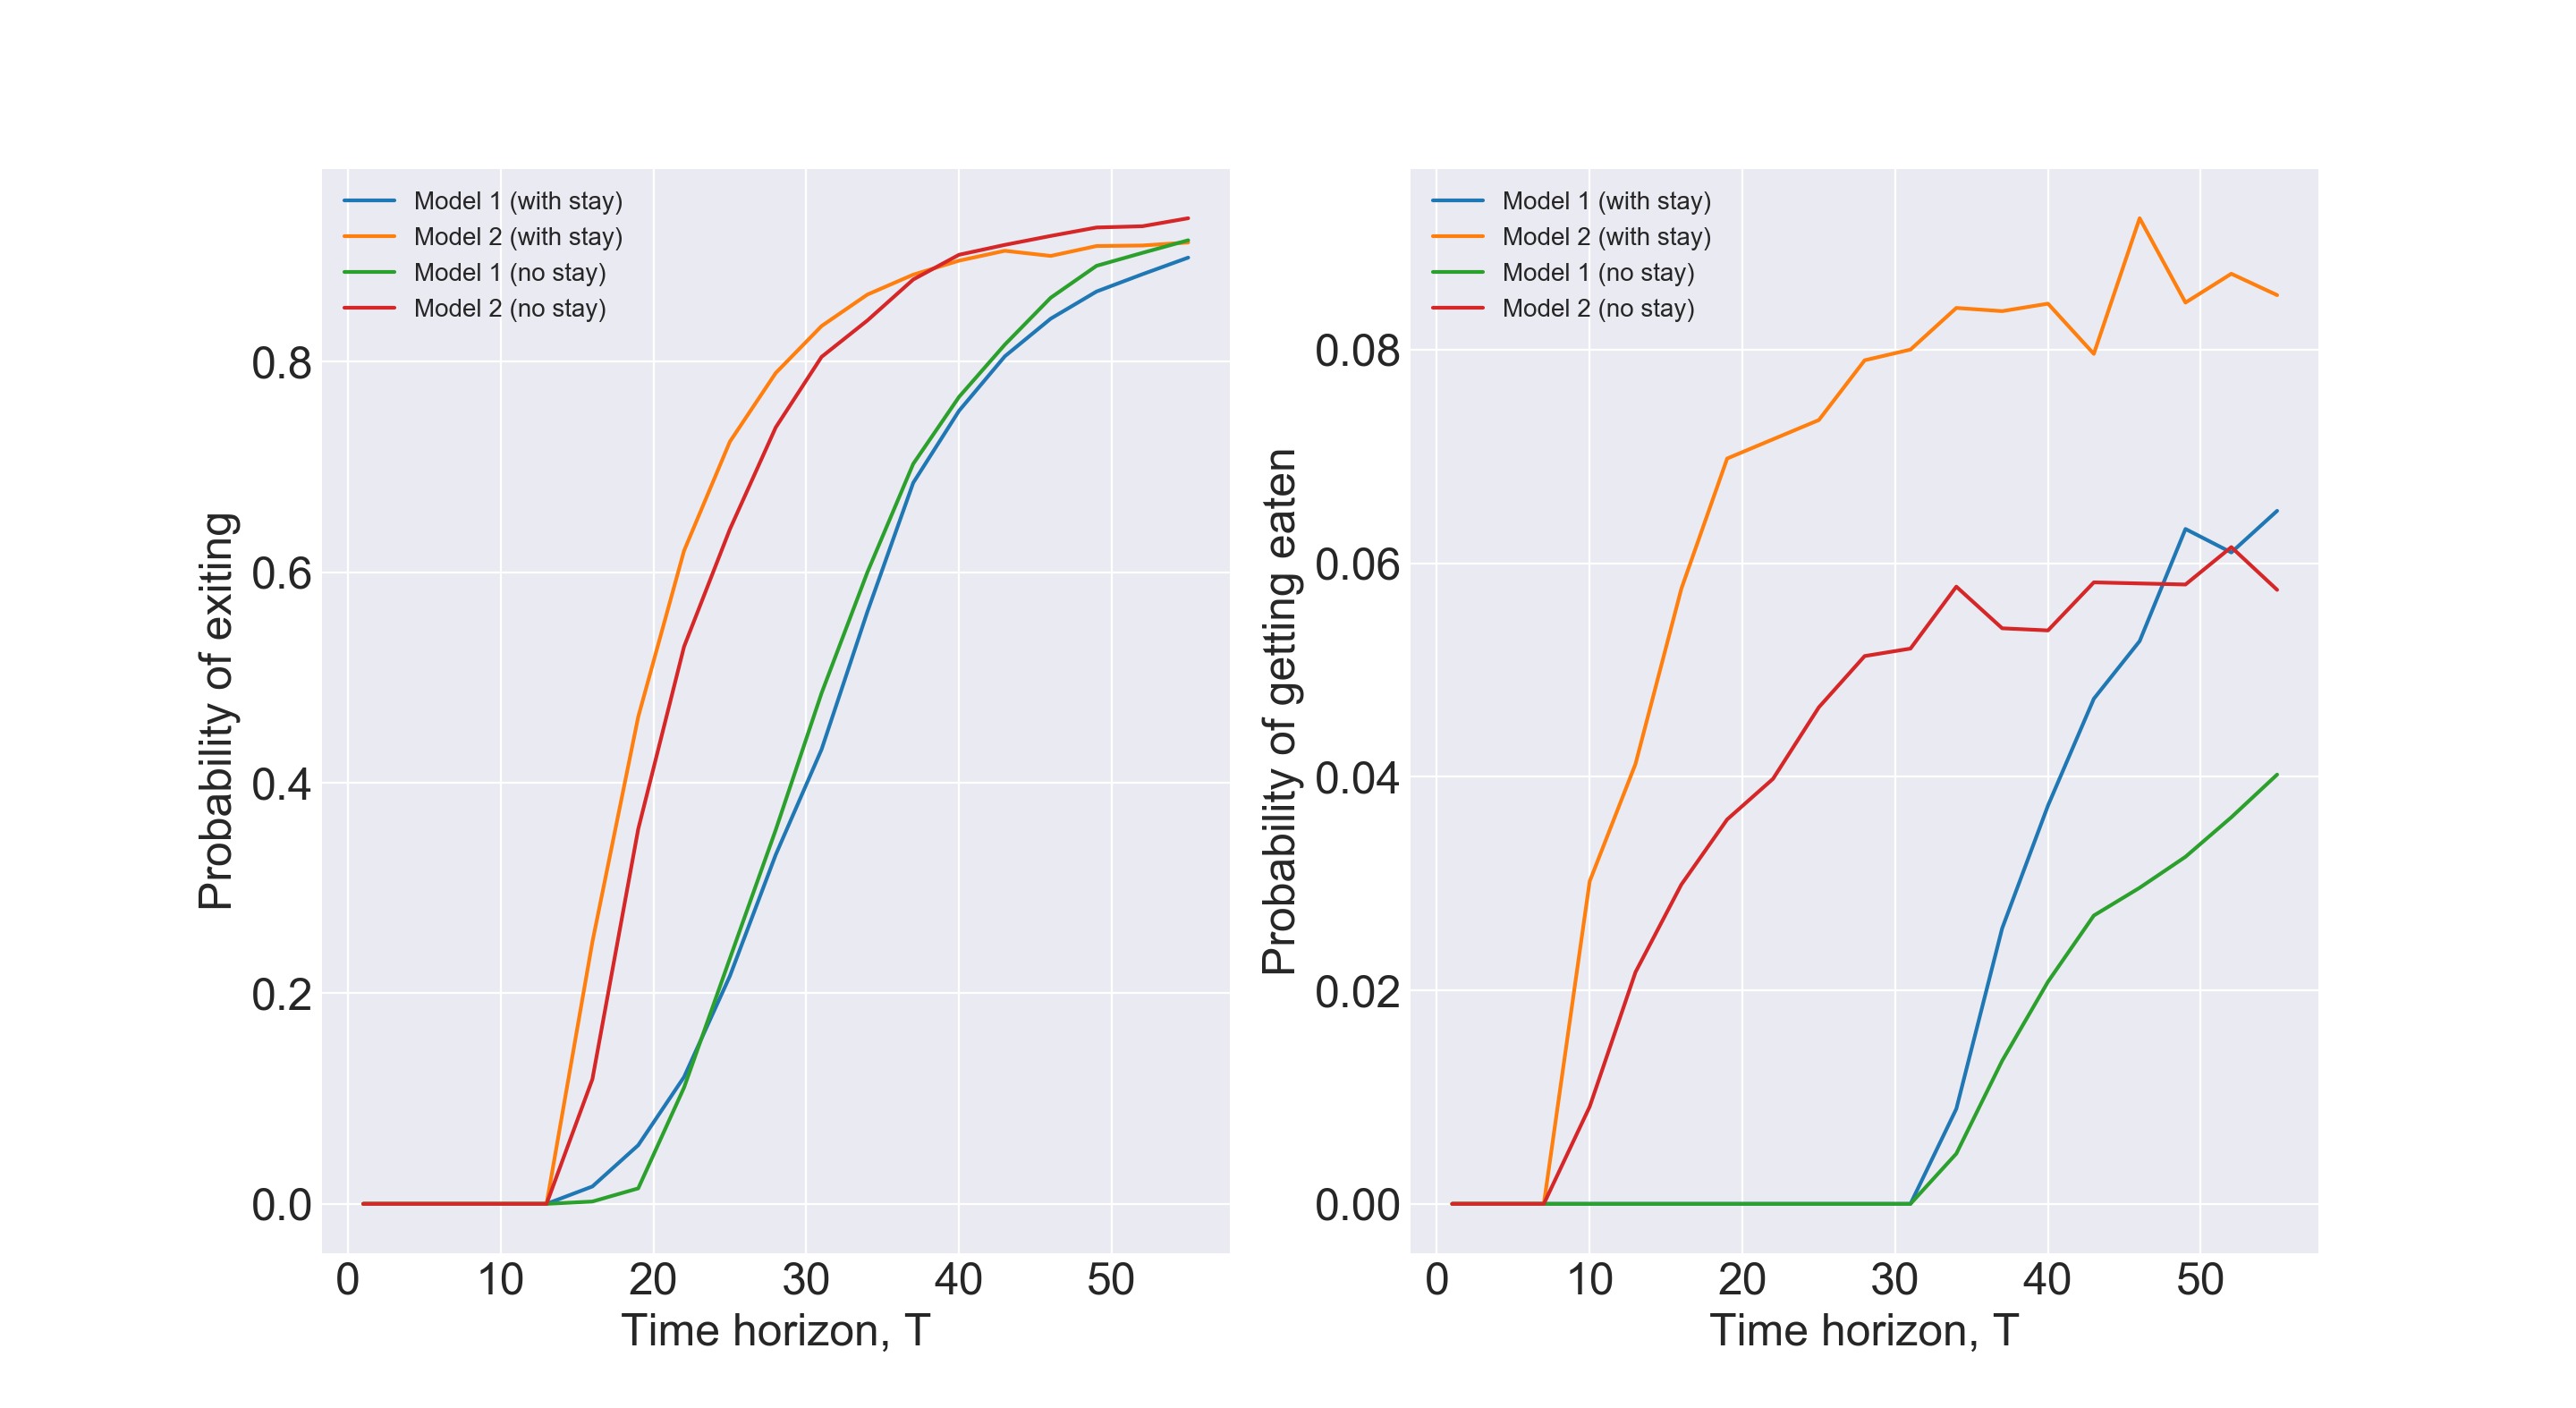
\includegraphics[width=\linewidth]{img/1b.png}
  \caption{The probability of exiting the maze on the left and the probability of getting eaten on the right. For the two different models and scenarios for minotaur movememnt.}
  \label{fig:1b}
\end{figure}

The result shows that, with respect to the probability of existing, the difference between allowing the minotaur to stay or not is small. However, Model 2, where the minotaur is modelled in the probabilities, performs better than Model 1 where the minotaur is modelled in the reward. This can be explained by the fact that modelling the minotaur in the reward (model 1) makes the player avoid getting near the minotaur as much as possible to avoid a negative reward, thus it takes the player a longer time to achieve the goal and thus it requires longer time horizon. In model 2 the player is more aggressive and takes the chance of getting near the minotaur.

When studying probability of getting eaten, it is clear that whether the minotaur can stay or not does indeed make a difference. We still find that the more aggressive Model 2 does perform better in both cases. For the same reasons mentioned above. Furthermore, we find that the probability of being eaten is lower if we do not allow the minotaur to stay. This can be explained by the fact that the uncertainty in the minotaur's movement is lower since it ends up in a certain state with a probability of $\frac{1}{4}$ as opposed to the lower certainty in position $\frac{1}{5}$, when we allow the minotaur to stay, that increases the chances of avoiding the minotaur successfully and, thus, have lower probability of getting eaten.

From Figure \ref{fig:1b} we also find that the optimal time horizon is around 60, since all models converge to the same probability of exiting, if T=60.

\subsection{c) Solving the problem using value iteration}
Assuming that our life is geometrically distributed with mean 30 based on

\begin{equation}
    \mathbb{E}(X) = \frac{1}{1-\lambda}
\end{equation}

We come to the conclusion that for this case $ \lambda = \frac{29}{30} $
The objective of this problem is to learn the policy that ensures the player reaches the goal in as few steps as possible. This is done by modifying the reward according to the following new formulation

\begin{itemize}
    \item If at state $s$, taking action $a$ leads to a wall or an obstacle then $r(s,a) = -\infty$
    \item If at state $s$, taking action $a$ leads to the minotaur then $ r(s,a) = -80 $
    \item If at state $s$ and $s$ is goal $r(s,a)=0$ 
    \item If at state $s$ and is at the same cell as the minotaur $r(s,a)=-80$ 
    \item If at state $s$ and previous state was with the minotaur, $r(s,a)=0$
    \item If at state $s$, taking action $a$ leads to the exit then $ r(s,a) = 0 $
    \item If at state $s$, taking action $a$ leads to neither of the aforementioned states $ r(s,a) = -1 $
\end{itemize}



\begin{table}[h!]
    \centering
    \caption{The expected time to reach the goal given the two different reward set ups}
    \begin{tabular}{c|c}
    Reward & Expected time \\ \hline
    Old reward model &  27.6 \\
    New reward model & 14.7
    \end{tabular}
\end{table}

With this model since reaching the minotaur is only penalized for the first time it happens the player is less risk averse and, thus gets to the goal quicker.


\section{Problem 2: Robbing Banks}
\subsection{a) MDP formulation}
\subsubsection{State space}
We define a state as a tuple (i,j,k,l) where the first two parameters describe the position of the player in the grid and the last two that of the police. Any position outside the grid is called an $impossible$ $state$. The formal definition of the state space is given below.

\begin{equation} 
\label{state_space_1}
\mathcal{S} = \Big\lbrace (i,j,k,l) ~:  (i,j, k, l) \textrm{ is not an impossible state}  \Big\rbrace
\end{equation}

\subsubsection{Action space $\mathcal{A}$}
The action space is defined as 
\begin{equation}
    \mathcal{A} = \{stay, up, down, left, right \}
\end{equation}
where each action corresponds to the movement that the player takes.
\subsubsection{Transition probabilities $\mathcal{P}$}
The transition probabilities for the model are formulated as the following

\begin{itemize}
  \item $\mathbb{P}(0,0,1,2|i,j,k,l,a)=1 \textrm{, if } i=k \textrm{ and } j=l, \forall a$. When the player is caught by the police, the game restarts regardless of what action the player takes.
  \item $\mathbb{P}(s'|s,a)=0 \textrm{ if } s' \textrm{ is an impossible state }$. When at state $s$, the player cannot take a given action $a$ and end up in an impossible state, instead it stays in the same place.
  \item $\mathbb{P}(s'|s,a)=\frac{1}{\# \textrm{actions by police}}$, for $s'$ all possible states that the game can end up in after player takes action $a$ and the police move according to the description in the exercise which depends on the relation between the position of the police and the player. Where \textit{\# actions by police} is $2$, if after taking action $a$ the  player ends up in a state where $i \neq k$ and $j \neq l$. Otherwise if the player ends up in a state where $i=k$ or $j=l$, then \textit{#actions by police}$=3$.
  \item $\mathbb{P}(s'|s,a)=0$, otherwise.
\end{itemize}

\subsubsection{Rewards $\mathcal{R}$}
The rewards for the model are defined as follows 
\begin{itemize}
    \item If at state $s$, taking action $a$ leads to an impossible state, then $r(s,a) = -\infty$
    \item If at state $s$, taking action $a$ leads to a bank, then  $ r(s,a) = 10 $
    \item If at state $s$, and taking action $a$ leads to getting caught (moving into the same cell as police), then $r(s,a)=-80$  
    \item If at state $s$ and $i=k$ and $j=l$, i.e. the police has moved into our cell, then $r(s,a)=-80$  
    \item If at state $s$, taking action $a$ leads to neither of the aforementioned states $ r(s,a) = 0 $
\end{itemize}

\subsection{b) The value function}
The problem was solved using value iteration. In this part we study the value function as a function of the discount factor $\lambda \in (0,1)$, at the initial state $s=(0,0,1,2)$, as presented in Figure \ref{fig:q2-vfdiff}. Furthermore, we study the policy for different values for the discount values at states $s=(i,j,0,0)$.

\begin{figure}[h!]
    \centering
    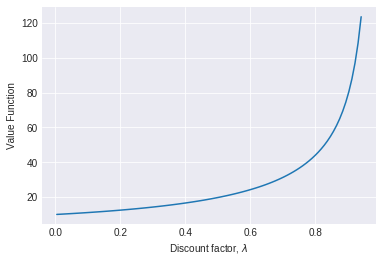
\includegraphics[width=0.6\linewidth]{img/value_function_different_lambda.png}
    \caption{The value function at the initial state $s=(0,0,1,2)$ as a function of $\lambda$}
    \label{fig:q2-vfdiff}
\end{figure}

 As can clearly be seen in \ref{fig:q2-vfdiff} the value function for the initial state increases with lambda. This can be explained by the fact that the lower $\lambda$ is the less we consider the rewards of future steps, and since the player never gets caught and most of the time stays at a different bank, it corresponds to a high positive value. On the other hand, if $\lambda \approx 0$ the value function is approximately as big as the reward gained for staying at the inital state which coincides with one of the a bank,  $V^*(s) \approx r(s,a)$. Thus, the rewards is as big as the one gained for staying at the bank and no more, since the value function, then, doesn't consider any future states due to the small discount factor.

\begin{figure}[h!]
    \centering
    \subfigure[$\lambda=0.2$]{
        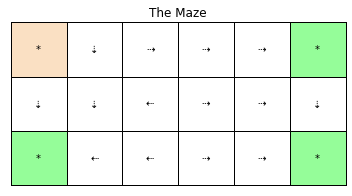
\includegraphics[width=0.4\linewidth]{img/lambda_0_2.png}
    }
    \subfigure[$\lambda=0.4$]{
        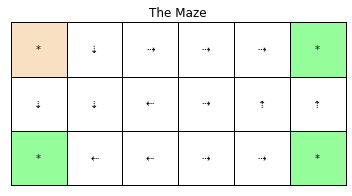
\includegraphics[width=0.4\linewidth]{img/lambda_0_4.png}
    }
    \subfigure[$\lambda=0.6$]{
        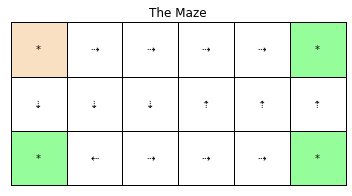
\includegraphics[width=0.4\linewidth]{img/lambda_0_6.png}
    }
    \subfigure[$\lambda=0.8$]{
        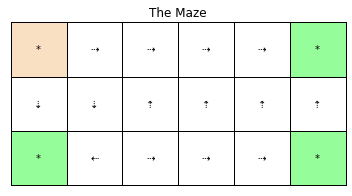
\includegraphics[width=0.4\linewidth]{img/lambda_0_8.png}
    }
    \caption{The policy for state state$s=(i,j,0,0)$ given different values for the discount factor $\lambda$}
    \label{fig:q2-grid}
\end{figure}

In Figure \ref{fig:q2-grid} we observe that for lower discount factors the optimal policy tells the player to move towards the bank that is closest to it. However, increasing the discount factor allows the player to look further into the future which explains why in the Figures the player tends towards banks that aren't necessarily closer. On the other hand, given a larger long term reward, since the player than is also aware of the fact that the police will take longer to catch up to him/her, leads to the player preferring banks further away from the police.

\newpage
\section{Problem 3: Bank Robbing (Reloaded)}
\subsection{a) Q-learning}
In this part we study the convergence of the Q-learning algorithm, given the problem in the exercise, at the initial state $s=(0,0,3,3)$
We use the same action space as in Problem 2, and the sampled rewards for every action are sampled in a similar manner too, but with slightly different values. 

\textbf{Reward $\mathcal{R}$}
\begin{itemize}
    \item If at state $s$, taking action $a$ leads to an impossible state, then $r(s,a) = -\infty$
    \item If at state $s$, taking action $a$ leads to a bank, then  $ r(s,a) = 1 $
    \item If at state $s$, taking action $a$ and letting the police take a random move leads to getting caught then $r(s,a)=-10$  
    \item If at state $s$ and $i=k$ and $j=l$, i.e. the police has moved into our cell, then $r(s,a)=-10$  
    \item If at state $s$, after taking action $a$ and letting police move randomly leads to neither of the aforementioned states $ r(s,a) = 0 $
\end{itemize}

We find in figure \ref{fig:q3-q-learn} that the Q-learning algorithm converges to a value of $V(s)\approx 37$ after $1.5$ million iterations.

\begin{figure}[h!]
    \centering
    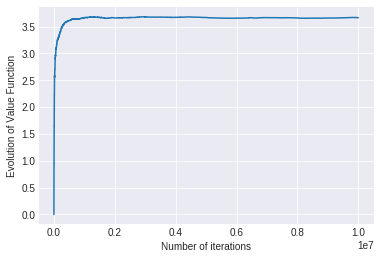
\includegraphics[width=0.6\linewidth]{img/Q_learning.png}
    \caption{The evolution of the value function at the initial state $s=(0,0,3,3)$ for Q-learning}
    \label{fig:q3-q-learn}
\end{figure}

\subsection{b) SARSA}
For SARSA, the reward function is exactly the same as Q-learning. The only difference now is that we do SARSA in an $\epsilon$-greedy manner. We take an exploring action with probability $\epsilon$ and with probability $1-\epsilon$ we perform the action suggested by the most recent policy. In Figure \ref{fig:q3-sarsa} we can see the obtained result, when studying different values for $\epsilon$.

As seen in Figure \ref{fig:q3-sarsa} the Value Function converges to lower values with increasing $\epsilon$. While it is lower than the values, the Q-learning converged to, under no means does it mean that the agent has not learned. For example for the case where $\epsilon = 0.1$ both algorithms converge towards the same policy. 
The Value Function presented in Figure \ref{fig:q3-sarsa} depends heavily on the random actions that are taken once in a while through the $\epsilon$-greedy policy, independent of the base policy. This can be seen in the fluctuations of the Value Function which are of higher frequency the bigger $\epsilon$ gets. The often we explore the often we are prone to mistakes and the smaller the value we tend to converge to is. 
In addition to that we concluded that one cannot derive convergence by only observing the Value Function evolution of the  $\epsilon$-greedy policy. For that we would need to decay $epsilon$ or use some other action choice mechanism that reduces exploration over time.

\begin{figure}[H]
    \centering
    \subfigure[$\epsilon=0.1$]{
        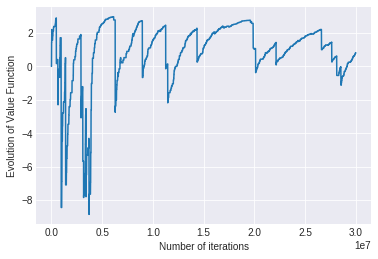
\includegraphics[width=0.4\linewidth]{img/SARSA_0_1}}
    \subfigure[$\epsilon=0.2$]{
        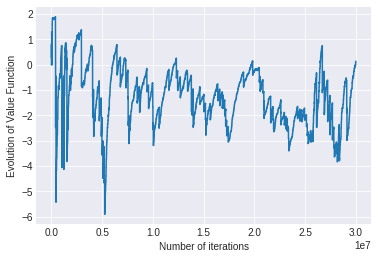
\includegraphics[width=0.4\linewidth]{img/SARSA_0_2}}
    \subfigure[$\epsilon=0.3$]{
        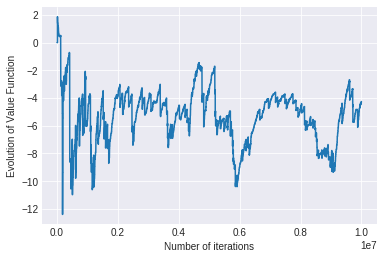
\includegraphics[width=0.4\linewidth]{img/SARSA_0_3}}
    \subfigure[$\epsilon=0.4$]{
        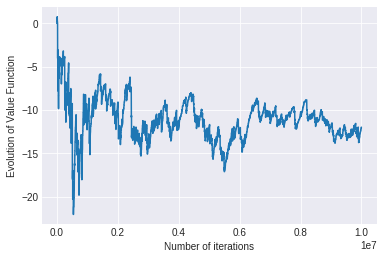
\includegraphics[width=0.4\linewidth]{img/SARSA_0_4}}
    \subfigure[$\epsilon=0.5$]{
        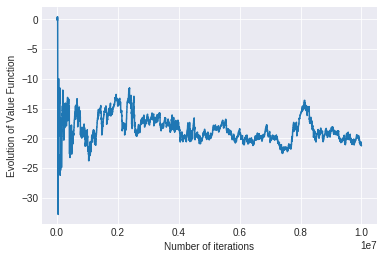
\includegraphics[width=0.4\linewidth]{img/SARSA_0_5}}
    \caption{The evolution of the value function at the initial state for different values of $\epsilon$ using SARSA with 20 000 000 iterations.}
    \label{fig:q3-sarsa}
\end{figure}



In conclusion we can say that Q-learning's big strength is directly learning the optimal policy, but it does so at the expense of being more likely to make certain kinds of error, whereas SARSA's strength is that it will better optimise the values seen whilst learning, but it does this at the expense of not learning the optimal policy directly.
\end{document}